\chapter{Experiential Learning of Networking Technologies: Understanding TCP States -- Part 2}

\begin{center}
\uppercase{Ram P. Rustagi}

\vskip -7pt

Department of CSE, KSIT Bangalore

\bigskip

\uppercase {Viraj Kumar}

\vskip -7pt

Divecha Centre for Climate Change, IISc Bangalore
\end{center}

\noindent\makebox[\textwidth]{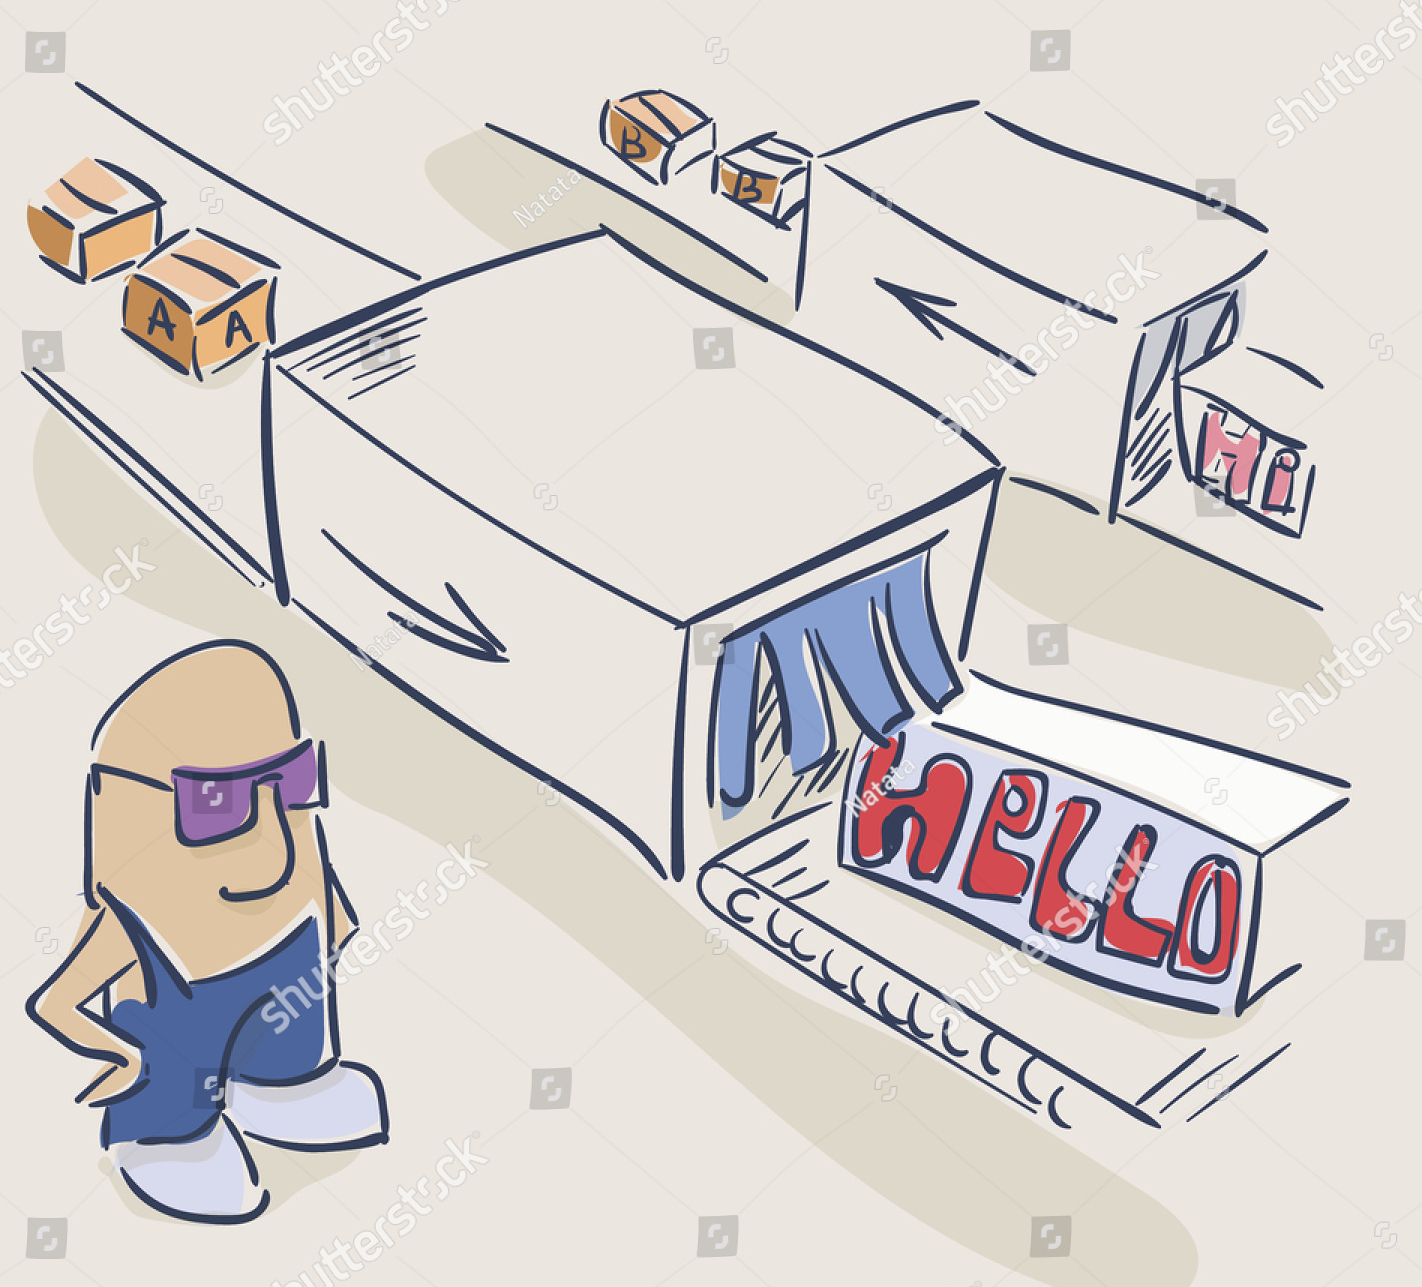
\includegraphics[width=\paperwidth,height=16cm]{src/Figures/chap3/stock-vector-presentation-layer-osi-model-vector-illustration-333711977.jpg}}

\newpage

\begin{multicols}{2}

\setcounter{figure}{0}
\section*{Abstract}

This article focuses on the states of a TCP connection once one of the endpoints decides to terminate the connection. This so-called teardown phase involves the exchange of numerous messages (for reasons we will explore), and the TCP connection itself transitions through several states. Web developers often have only an overly simplistic understanding of these states, which may suffice when the network behaves reliably. However, a deeper understanding of TCP states is essential to design web applications that robustly manage TCP connections even in the presence of network faults during the teardown phase, and debug poorly design applications that exhibit poor resource utilization and poor performance in such situations. As always, we will explore these issues through a series of experiential learning exercises.

\section{Introduction}


In the last article \cite{chap3-key8}, we discussed the three phases of TCP \cite{chap3-key1} communication: (1) connection setup, (2) data transfer, and (3) teardown. For each TCP connection, the two machines communicating via this connection independently maintain information about the present state of this connection from their own perspective (one of the 11 possible states listed in Table \ref{chap3-tab1}). The last column of this table lists the states of a TCP connection after one of the machines decides to close the connection by initiating connection termination. In case of any abnormal network behaviour, an understanding of these states of the TCP connection is critical to accurately diagnose problems and resolve them.

For experiential understanding of these TCP states and the Transport layer \cite{chap3-key2}, we need a basic setup consisting of two machines $H_{1}$ and $H_{2}$ connected via a network as shown in Figure \ref{chap3-fig1}. We will make use of i) a network utility called \textit{netcat} (nc) \cite{chap3-key5}\cite{chap3-key6} that can be used to create both a TCP client and a TCP server (for the latter, run with the option $-1$), ii) a utility to implement firewalls functionality called \textit{iptables} \cite{chap3-key7}, and iii) some custom applications (simple Python programs) to depict the typical application behaviour.

As extensively discussed in \cite{chap3-key8}, the two machines exchange messages during connection setup (Phase 1) and data is transferred during Phase 2 when both machines ``agree'' that the TCP connection state is ESTABLISHED.
\end{multicols}

\begin{table}[!ht]
\centering
\caption{TCP Connection state in various phase of communication}\label{chap3-tab1}
\smallskip
\renewcommand{\arraystretch}{1.4}
\begin{tabular}{|c|c|c|c|}
\hline
\textbf{Initial (no connection)} & \textbf{Phase 1 Connection Setup} & \textbf{Phase 2 Data Transfer} & {\bf Phase 3 Connection Tear Down}\\
\hline
CLOSED & LISTEN & ESTABLISHED & FIN\_WAIT\_1\\
       & SYN\_SENT & & FIN\_WAIT\_2\\
       & SYN\_RECV & & CLOSING\\
       &          & & TIME\_WAIT\\
       &          & & CLOSE\_WAIT\\
       &          & & LAST ACK\\
\hline
\end{tabular}
\end{table}

\begin{figure}[!htb]
\centering
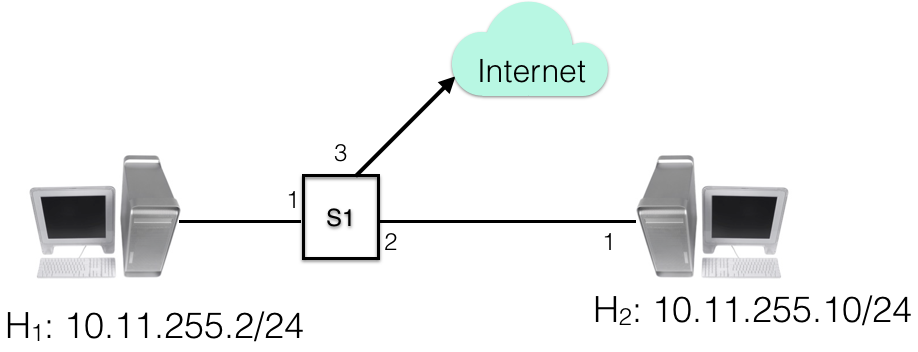
\includegraphics[scale=.43]{src/Figures/chap3/1.jpg}
\caption{Basic setup of conducting TCP learning exercises}\label{chap3-fig1}
\end{figure}

\begin{multicols}{2}
\section{TCP Teardown (Phase 3)}

At some point during Phase 2, one of the applications will decide that it does not need to transmit data any more and will initiate connection closure (i.e., the TCP connection will enter the teardown phase, Phase 3). This application (which can be either the client or the server application) will follow the \textit{Active Close} path in Figure \ref{chap3-fig2} (shown on the left in purple colour), and the other application will follow the \textit{Passive Close} path (shown on the right in orange colour). Each sent message is identified by a number in parentheses ($n$), and when this is received it is identified as ($n'$). It should be noted that even though connection initiation (connection setup in Phase 1) is always by a client, connection termination can be initiated by either the client or the server (or by both at the same time -- a very rare case that is generally not seen in real-life applications).

To understand why so many states are necessary in Phase 3, note that data transfer may continue for a long time after connection closure is initiated. As a concrete example, consider a typical case of web communication where a web client is downloading a large file (e.g., an image or a document). After the client sends the URL details (which may correspond to only a few hundred bytes, including HTTP headers), it need not send any further data and it may decide to initiate TCP connection closure (to better manage client-side Operating System resources). Despite this, the application should continue to receive data until the server has sent the full file. The connection can only be closed after the server has sent the last byte (which could be for several minutes or even hours after the client’s initial request for closure) and has received the corresponding TCP-level acknowledgement (in accordance with TCP reliable delivery). Keeping in mind that some messages can be lost due to network faults, TCP states must maintain enough information to properly manage the connection. For ease of understanding, let us first consider the simpler (and more common) scenario when the network functions correctly.

\section{TCP Connection Closure\\ -- Normal case}

Phase 3 starts when either the client or the server application invokes the \textit{connection close} API. For clarity, we will assume that the application on $H_{1}$ initiates the connection close and $H_{2}$ responds to this connection close request. Thus, $H_{1}$ transmits a TCP FIN(ish) message (1) to $H_{2}$ and must wait for a response (typically an acknowledgement). Thus, the TCP connection on $H_{1}$ enters the state FIN\_WAIT1 which indicates that it has initiated connection closure by transmitting the FIN message and is waiting for a response. When $H_{2}$ receives this FIN message ($1'$), it responds with an ACK message (2) and the TCP connection on $H_{2}$ enters the CLOSE\_WAIT state. This state indicates that the other side has initiated connection closure and the same has been acknowledged by, but the connection should not be closed yet because the application running on $H_{2}$ may wish to transmit more data. When $H_{1}$ receives this ACK message ($2'$), the TCP connection on $H_{1}$ enters the state FIN\_WAIT2.


{\parfillskip=0pt
As long as the application running on $H_{2}$ has more data to send, the data will be sent over the connection (5) and it is received ($5'$) and acknowledged by $H_{1}$ (6). This acknowledgement will be received by $H_{2}$ ($6'$). As soon as the application running on $H_{2}$ determines that no more data is to be sent, it sends a FIN message (3). When this is received by $H_{1}$ ($3'$), the TCP connection state on $H_{1}$ moves from FIN\_WAIT2 to TIME\_WAIT and an ACK (4) is transmitted. Note that the TCP connection state on $H_{1}$ does not move directly to the CLOSED state because, as discussed in detail in \cite{chap3-key8}, it is necessary to ensure that no new connection with same TCP tuple (i.e. source IP address, source port number, destination IP address,\par}
\end{multicols}

\begin{figure}[!htb]
\centering
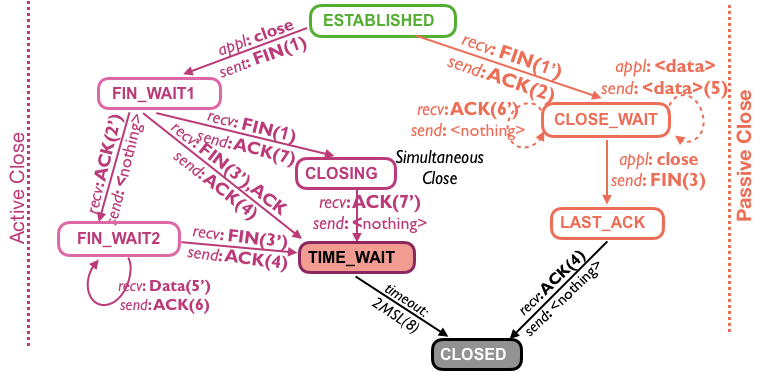
\includegraphics[scale=.55]{src/Figures/chap3/2.jpg}
\caption{TCP connection teardown phase}\label{chap3-fig2}
\end{figure}

\begin{multicols}{2}
\noindent
destination port number) is used until all packets corresponding to an earlier such connection could be lingering in the network. This waiting time is known as 2MSL (twice the maximum segment lifetime) and is typically 120s. Another reason is that if there is no TIME\_WAIT state (i.e., if $H_{1}$ directly enters the CLOSED state) and if the ACK (4) message gets lost, then $H_{2}$ will remain in the LAST\_ACK state until timeout occurs. When $H_{2}$ retransmits the FIN message again, there may be no connection state on $H_{1}$, and thus $H_{1}$ will respond with TCP Reset (indicating an error condition), which leads to ungraceful connection termination \cite{chap3-key8}.

Let us consider the typical case of TCP connection teardown, which occurs when there is no network abnormality (as is usually the case). Suppose the application running on $H_{2}$ invokes the \lstinline|close()| call. This application will follow the TCP state transitions corresponding to active close (left side of Figure \ref{chap3-fig2}) whereas the application on $H_{1}$ will follow the TCP state transitions corresponding to passive close (right side of Figure \ref{chap3-fig2}). Thus, $H_{2}$ will send the FIN (1) message and move its TCP connection state to FIN\_WAIT1. When $H_{1}$ receives the FIN ($1'$) message, it sends the ACK (2) message and moves its TCP connection state to CLOSE\_WAIT. When this ACK ($2'$) message is received by $H_{2}$, it moves to the FIN\_WAIT2 state. At this point, let us suppose that the application on $H_{1}$ has no further need for the connection. Thus, immediately after sending the ACK (2) message, it sends its own FIN (3) message and moves to the LAST\_ACK state. When $H_{2}$ receives the FIN ($3'$) message, it responds with ACK (4) and moves the state from FIN\_WAIT2 to TIME\_WAIT. When $H_{1}$ receives the ACK ($4'$) message, its releases all the resources associated with this connection and completely closes this connection. This is depicted by the CLOSED state, which essentially implies that no connection exists. However, the application on $H_{2}$ remains in the TIME\_WAIT state for 2MSL (two times Max Segment Lifetime), as discussed in detail in \cite{chap3-key8} and corresponding program details in \cite{chap3-key9}.  

In the screenshots below, the names of the machines $H_{1}$ and $H_{2}$ are part of the command prompts and are preceded by the date/time to show the order in which commands were issued. Command windows are also split into an upper and a lower panel to improve clarity. The upper panel in each figure shows the command to invoke the application, initiate data transfer, and connection termination whereas the lower panel is used to display the TCP connection state and any firewall rule(s) that need to be configured. We assume that all experiments begin with no firewall rules set. To ensure this, we recommend issuing the command \textbf{sudo iptables -F} on the machines before each experiment.

\medskip
\noindent
\textbf{Experiment 1:\\ TCP State transition for normal TCP application closure.}
\smallskip

The following experiment demonstrates this typical teardown scenario in Figure \ref{chap3-fig3} and Figure \ref{chap3-fig4}. In Figure \ref{chap3-fig3}, the application on $H_{2}$ moves the TCP connection state from LISTEN to ESTABLISHED and then, via intermediate transient states (as discussed above), to TIME\_WAIT as shown by the last line of the lower panel of this figure.

The states followed by the application on $H_{1}$ similarly shown in Figure \ref{chap3-fig4}. Thus, from the ESTABLISHED state, the TCP connection follows intermediate transient states of CLOSE\_WAIT and LAST\_ACK before completely releasing all the associated resource.
\end{multicols}

\begin{figure}[!htb]
\centering
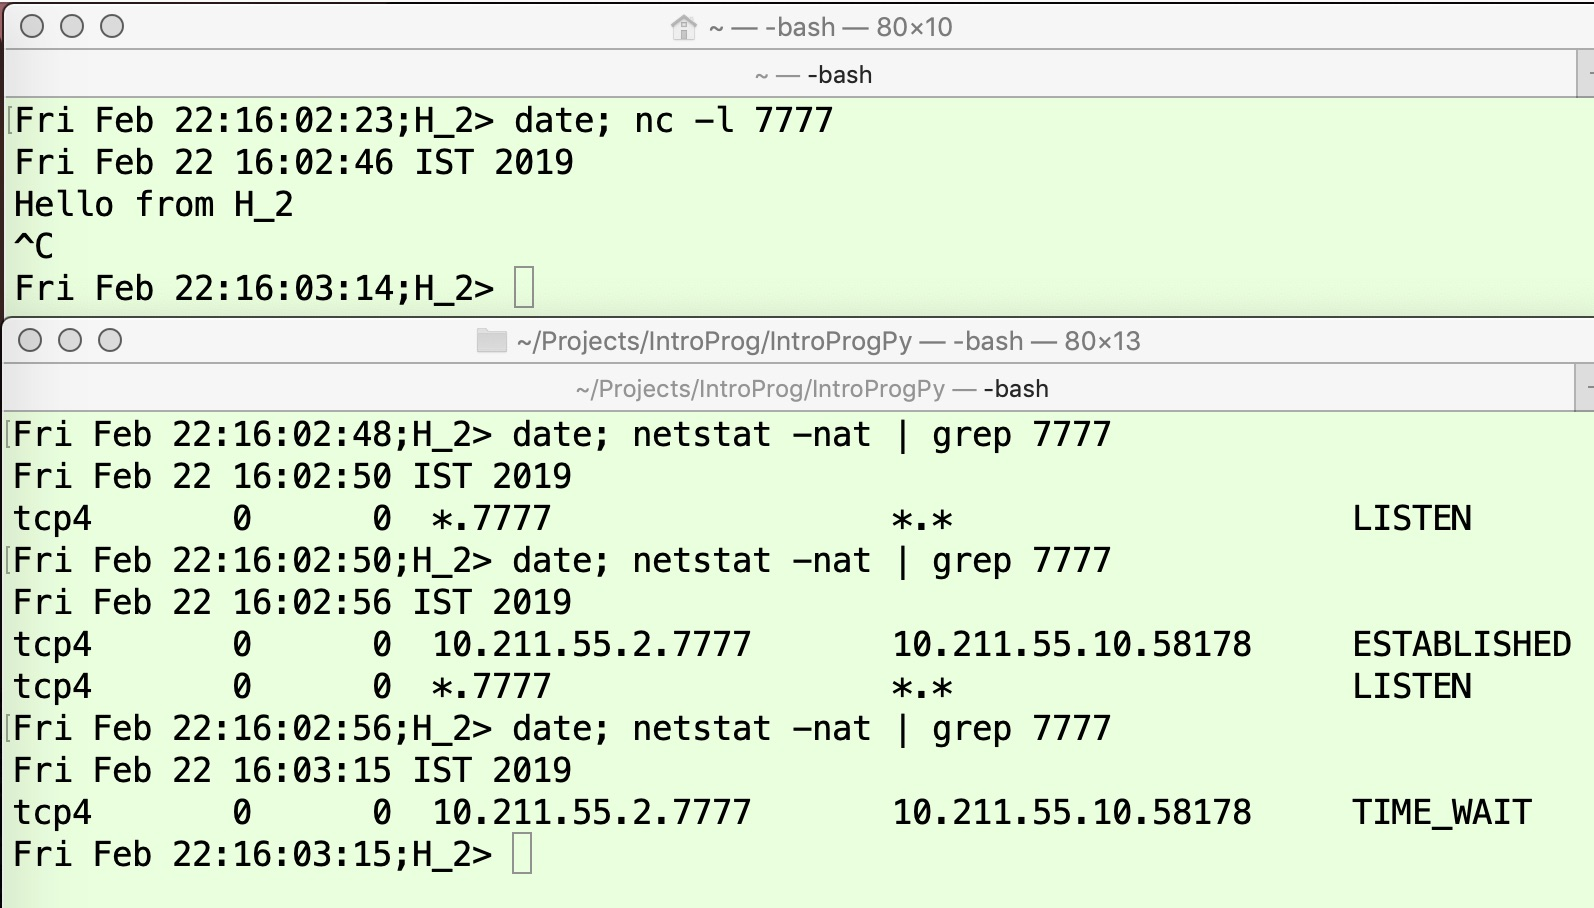
\includegraphics[scale=.25]{src/Figures/chap3/3.jpg}
\caption{TCP state for a general application initiating termination}\label{chap3-fig3}
\end{figure}

\begin{figure}[!htb]
\centering
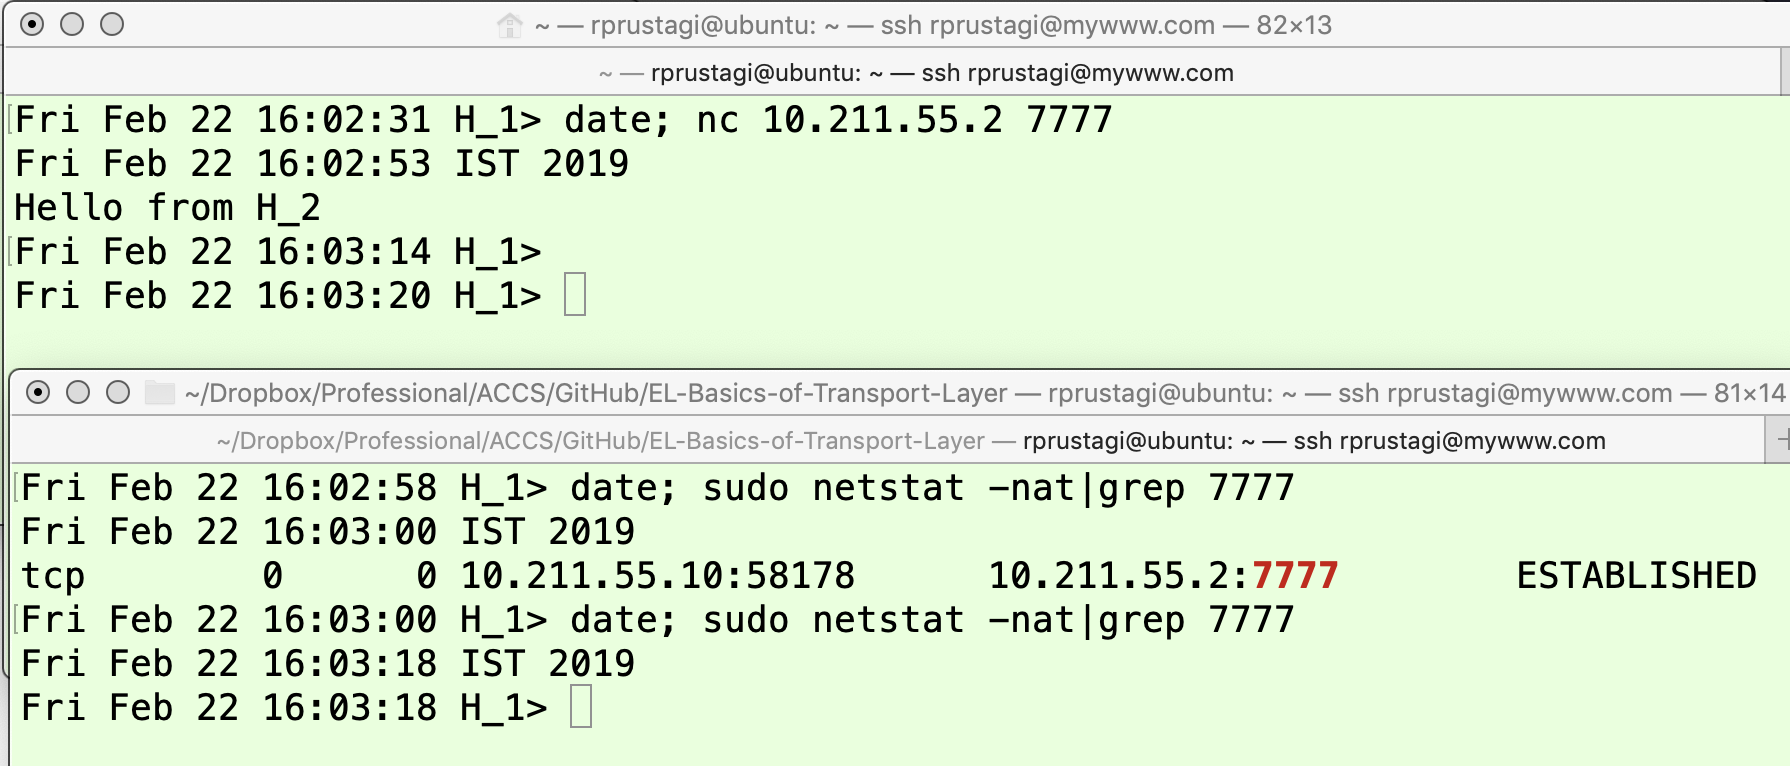
\includegraphics[scale=.45]{src/Figures/chap3/4.jpg}
\caption{TCP state for a general application receiving termination from other side}\label{chap3-fig4}
\end{figure}

\begin{figure}[!htb]
\centering
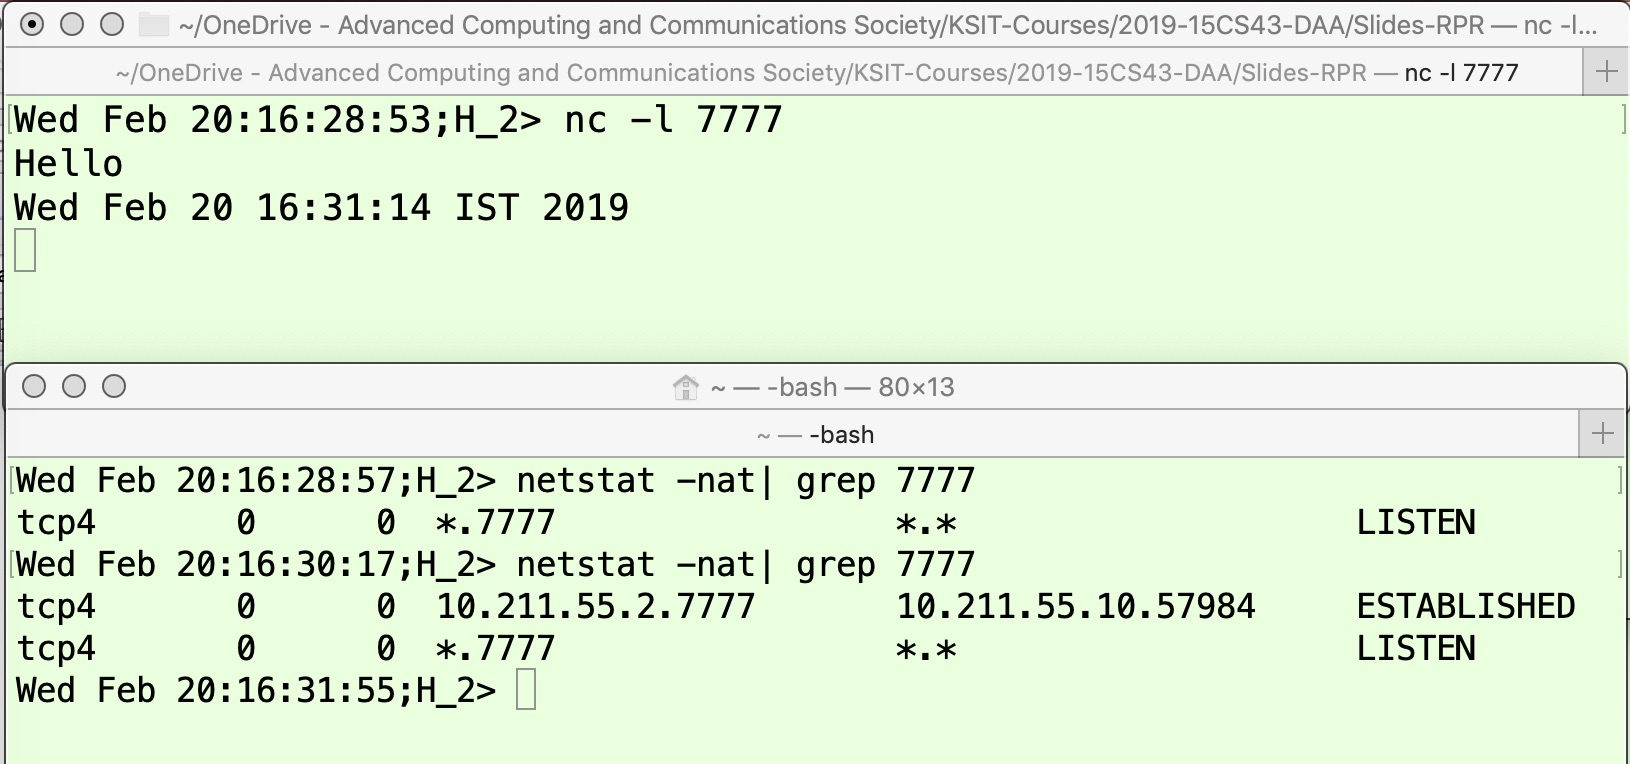
\includegraphics[scale=.25]{src/Figures/chap3/5.jpg}
\caption{Server states for understanding FIN\_WAIT1}\label{chap3-fig5}
\end{figure}

\begin{multicols}{2}
Under normal circumstances, the TCP connection closure follows the expected path and there is little reason for developers to have this detailed understanding of state changes. However, in some critical service function applications, the branding image and possibly the revenue of the service provider could be impacted if users perceive unsuccessful or delayed connection. For such applications, it is imperative that developers understand the details of various TCP termination states and the general conditions that lead to these states. We will now consider the situation where network failures during the teardown phase cause problems that can be diagnosed and rectified using our detailed understanding.

\section{TCP Connection Closure\\ FIN\_WAIT1 state}

\noindent
\textbf{Experiment 2:\\ TCP State FIN\_WAIT1 (\boldmath$H_{1}$) and ESTABLISHED ($H_{2}$)}
\smallskip

In the absence of network faults, when $H_{1}$ sends a FIN message and moves to state FIN\_WAIT1, it can expect to get an ACK almost immediately (i.e., within a few milliseconds) and thus move to state FIN\_WAIT2. Thus, to observe $H_{1}$ in the transient state FIN\_WAIT1, we need to simulate a network fault. As in our previous article \cite{chap3-key8}, we will make use of the \textit{iptables} utility to create abnormal network conditions.

In Figure \ref{chap3-fig2}, observe that $H_{1}$'s TCP connection state will remain in FIN\_WAIT1 if it sends a FIN message but does not receive an ACK. This can occur either because the FIN message was lost in the network or the FIN was received but the ACK did not reach the application initiating connection close. The upper panel in Figure \ref{chap3-fig5} shows an application on machine $H_{2}$ starting to run on TCP port 7777 at time 16:28:53, and the first line in the lower panel shows that the TCP connection state is LISTEN at time 16:28:57 (as described in detail in \cite{chap3-key8}). The application on machine $H_{1}$ connects to the application on machine $H_{2}$ at 16:30:22, as shown in the upper panel of Figure \ref{chap3-fig6}. The TCP connection state becomes ESTABLISHED, as shown by the output of the first command (issued at 16:30:41). Next, the text message ``Hello'' is exchanged, as shown in the upper panels of both these figures. To mimic the scenario where the FIN message is lost in the network, an iptables command is issued on $H_{1}$ to drop all FIN packets sent from $H_{1}$ with the destination port 7777 (shown by the third command in the lower panel of Figure \ref{chap3-fig6}). Now the application on $H_{1}$ is terminated by pressing Ctrl-C, as shown by the fourth line in the upper panel of Figure \ref{chap3-fig6}. When the TCP state is subsequently checked (fourth command in the lower panel of Figure \ref{chap3-fig6}), it is FIN\_WAIT1 at time 16:31:48. Since $H_{2}$ does not receive the FIN message (because of the \textit{iptables} command on $H_{1}$), the TCP connection remains in the ESTABLISHED state, as shown by the last command in the lower panel of Figure \ref{chap3-fig5} at 	time 16:31:55.

\medskip
\noindent
\textbf{Experiment 3:\\ TCP State CLOSE\_WAIT (\boldmath$H_{1}$) and FIN\_WAIT1 ($H_{2}$)}
\smallskip

Let us now consider the other possibility where $H_{1}$ receives the FIN message, but the ACK it sends back to $H_{2}$ as it moves to the CLOSE\_WAIT state (refer to Figure \ref{chap3-fig2}) gets lost. In this case, the TCP connection state on $H_{2}$ will continue to be FIN\_WAIT1. This scenario can be easily simulated by dropping the ACK message on $H_{2}$, as shown in Figure \ref{chap3-fig7} and Figure \ref{chap3-fig8}. In this experiment, when $H_{1}$ receives FIN it will send only the ACK (but not FIN) because we will assume that it still has some data to send. This functionality to send data even after receiving FIN from the other side cannot be achieved using the \textit{netcat} utility (this utility immediately sends a FIN/ACK as response when it receives a FIN message), so we have developed a simple Python program \textbf{tcp\_client.py} that sends the current date and time as the data at a specified time interval (option \textbf{-d}) for a specified number of times (option \textbf{-c}). This program can be accessed from \cite{chap3-key10}, and the key part of code is given in the Appendix.
\end{multicols}

\begin{figure}[!htb]
\centering
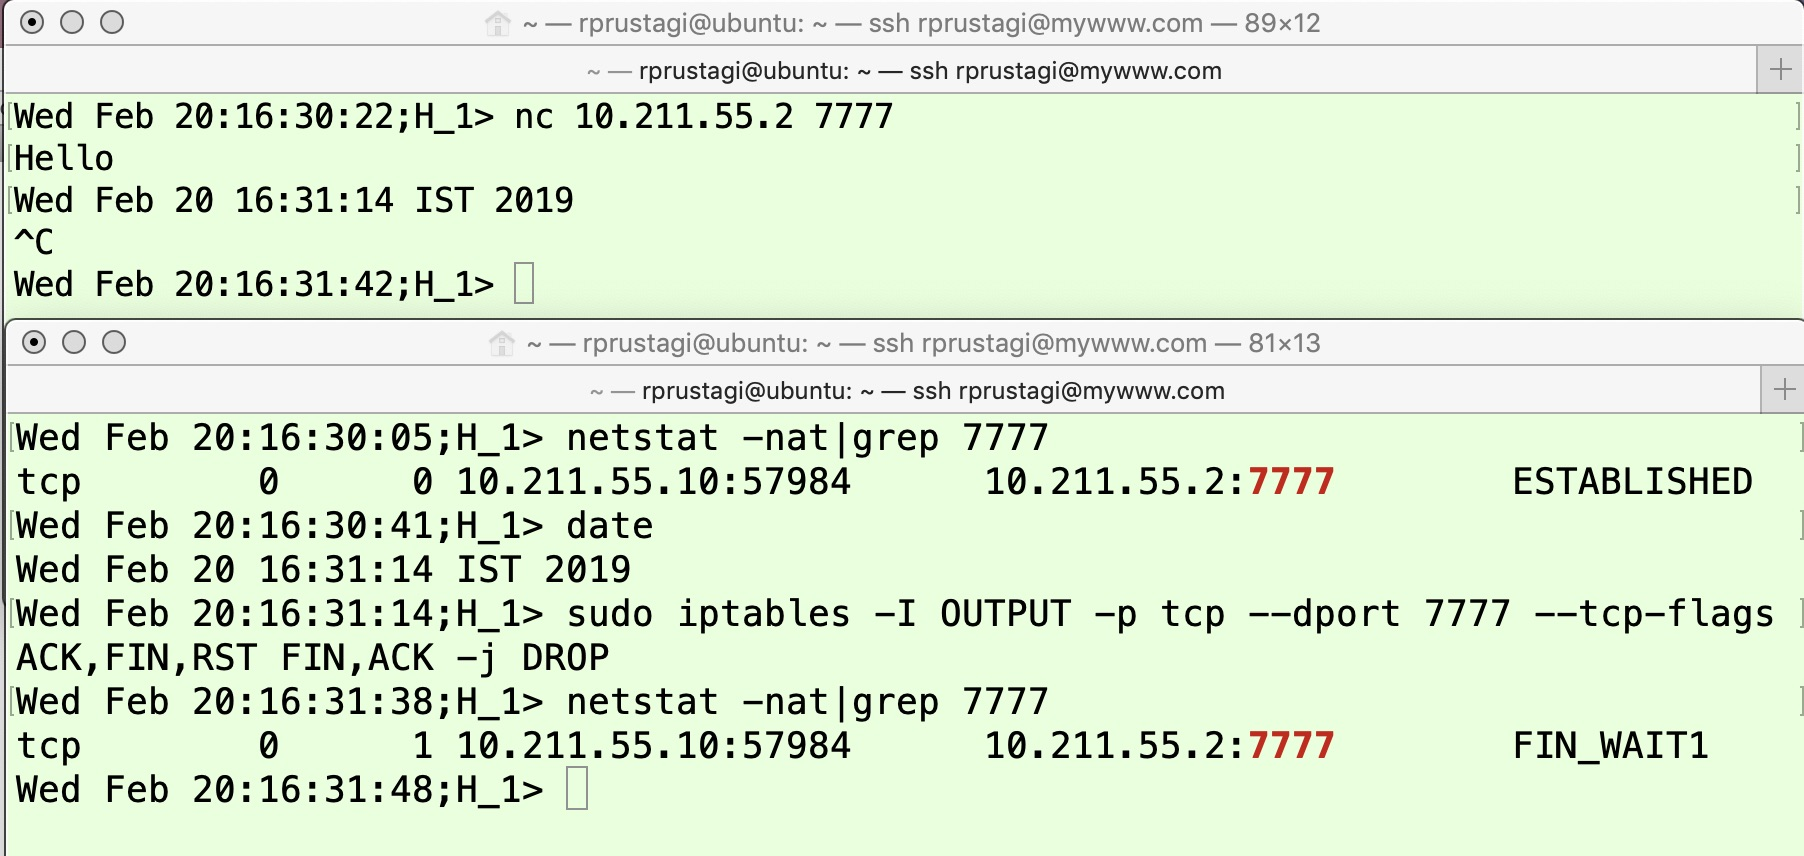
\includegraphics[scale=.22]{src/Figures/chap3/6.jpg}
\caption{Client state for understanding FIN\_WAIT1}\label{chap3-fig6}
\end{figure}

\begin{figure}[!htb]
\centering
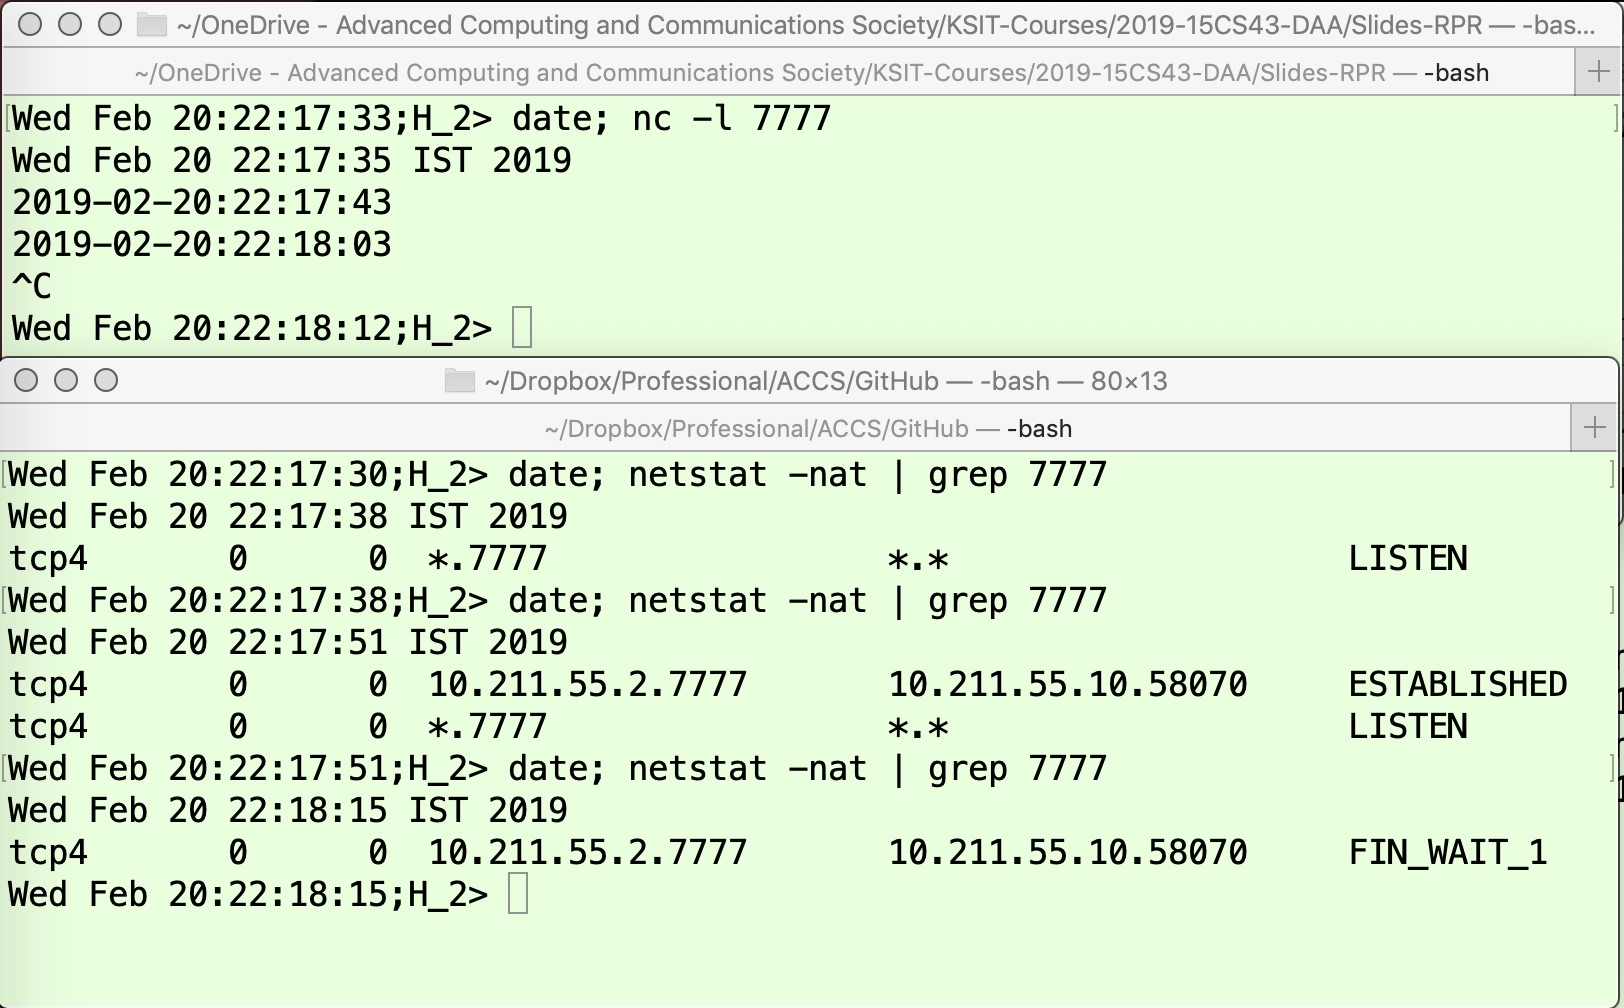
\includegraphics[scale=.241]{src/Figures/chap3/7.jpg}
\caption{Sending FIN but not receiving ack of FIN}\label{chap3-fig7}
\end{figure}

\begin{figure}[!htb]
\centering
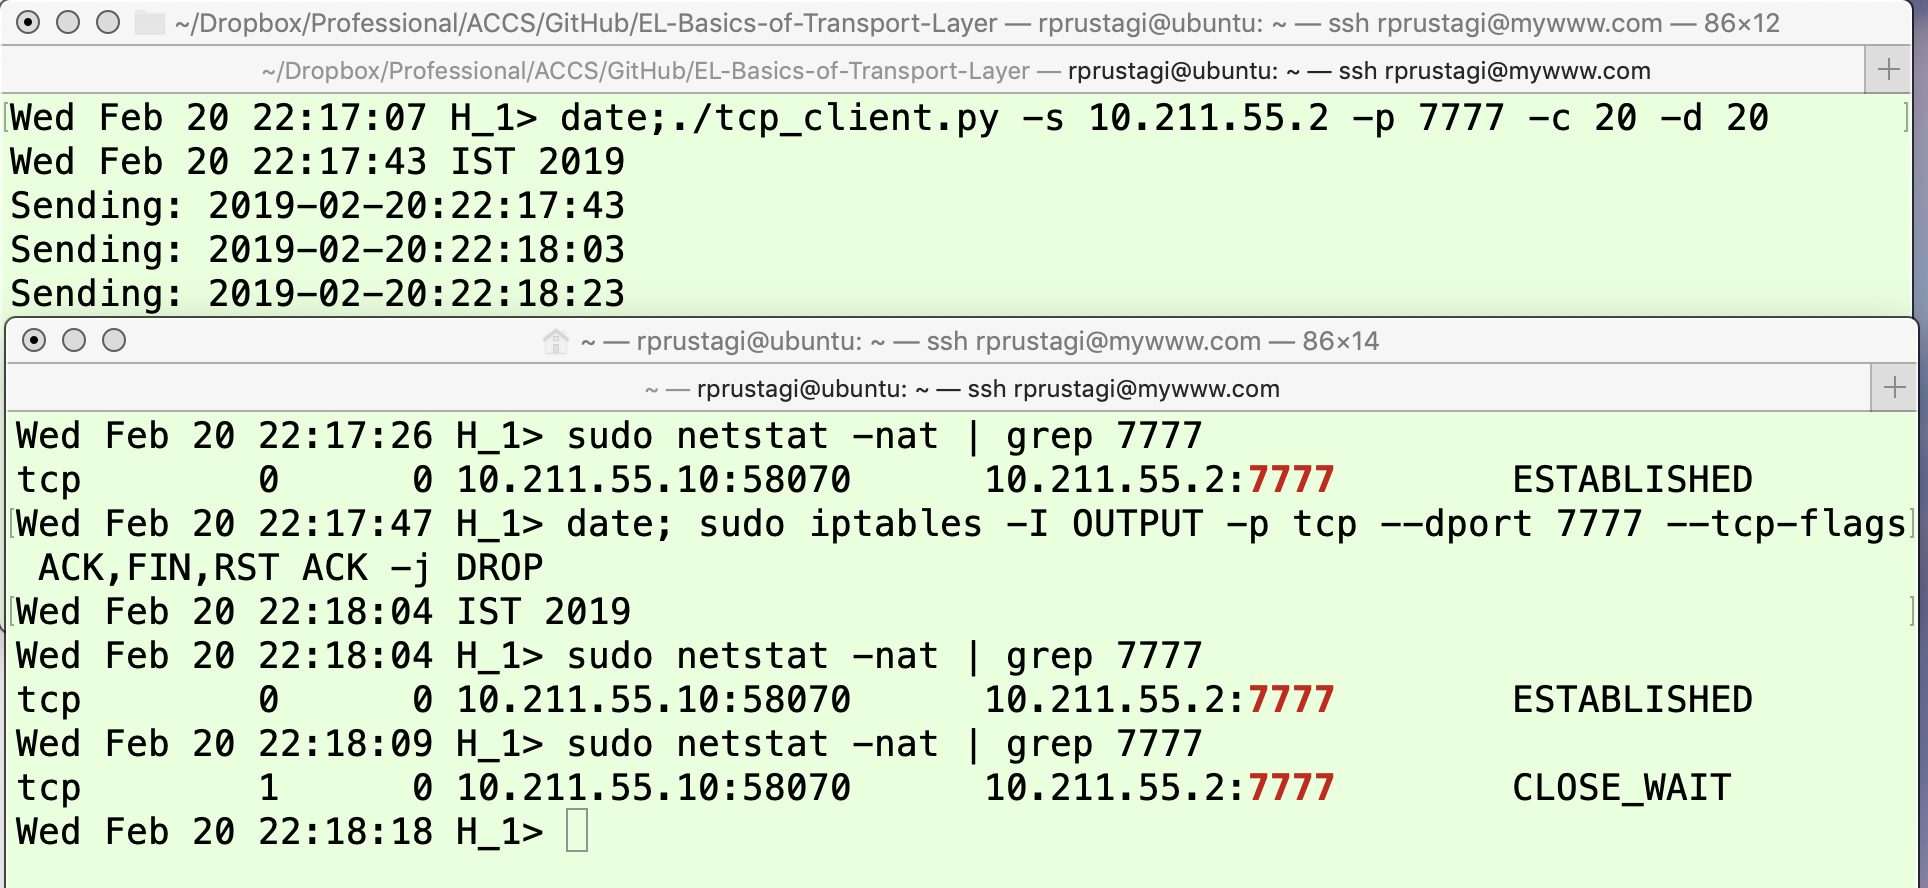
\includegraphics[scale=.42]{src/Figures/chap3/8.jpg}
\caption{Receiving FIN, sending Ack for FIN, Ack is lost}\label{chap3-fig8}
\end{figure}

\begin{figure}[!htb]
\centering
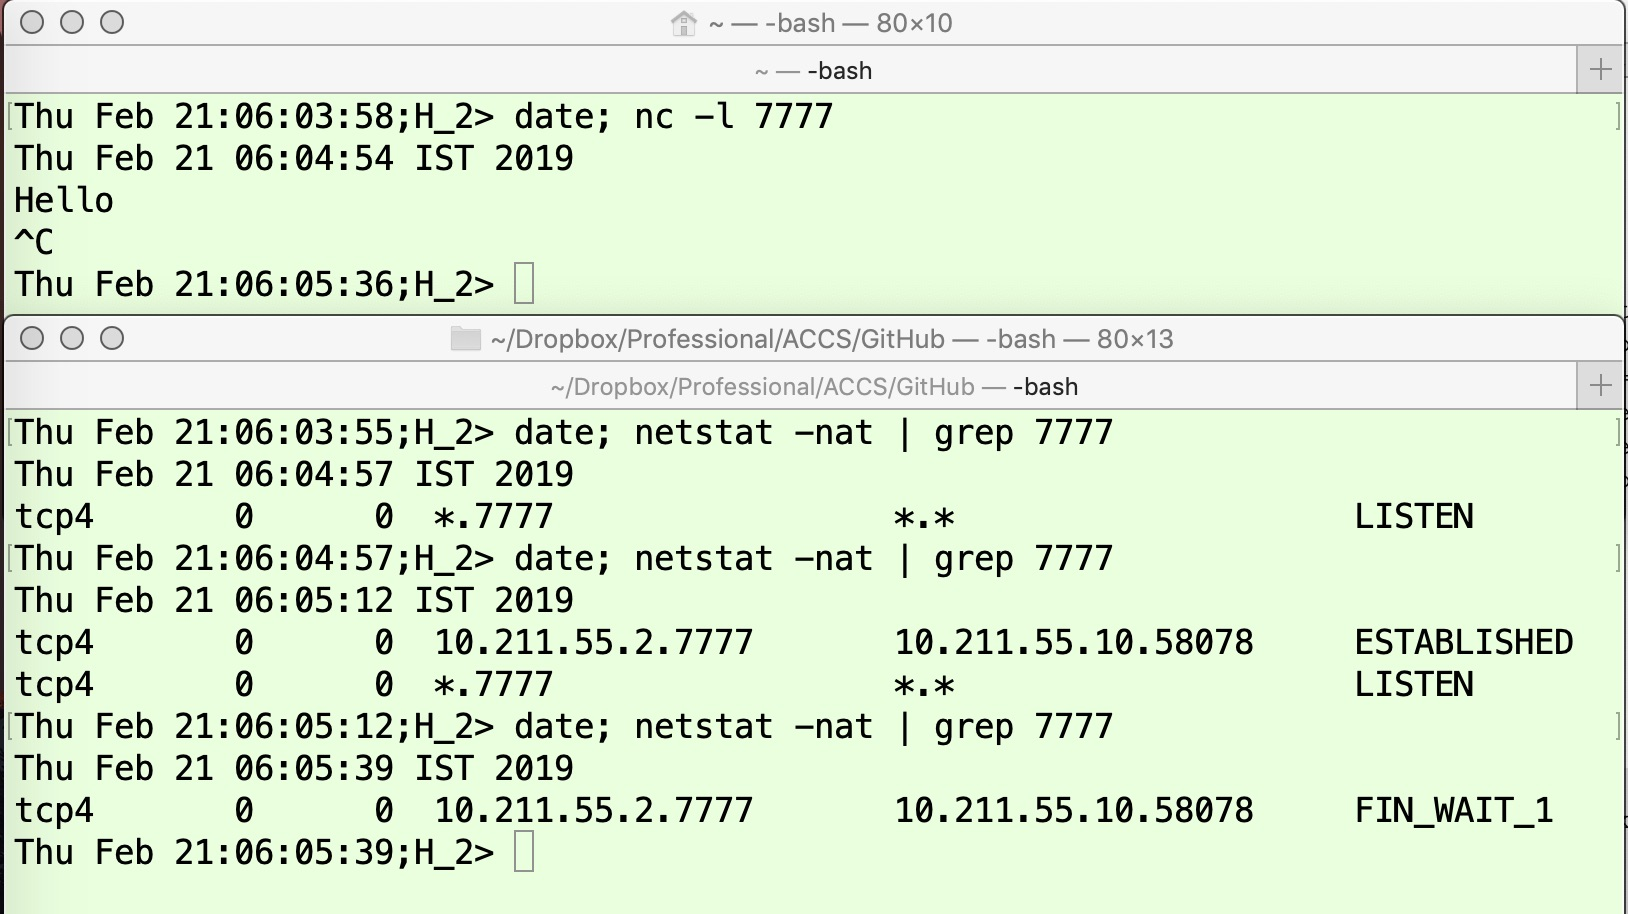
\includegraphics[scale=.228]{src/Figures/chap3/9.jpg}
\caption{Sending FIN, not receiving ACK}\label{chap3-fig9}
\end{figure}

\begin{multicols}{2}
The upper panel of Figure \ref{chap3-fig7} shows the data being received on $H_{2}$. The lower panel of this figure shows the TCP connection state on this machine, which starts from LISTEN (the output of the first \textit{netstat} command \cite{chap3-key3}\cite{chap3-key4}). Once the application on machine $H_{1}$ connects, the TCP connection state on $H_{2}$ changes to ESTABLISHED (output of the second command issued at time 22:17:51). Now, the application on $H_{2}$ is aborted using Ctrl-C, so it sends the FIN message and moves to state FIN\_WAIT1. The application on machine $H_{1}$ is shown in the upper panel of  Figure \ref{chap3-fig8}. The lower panel shows the TCP connection state as well as firewall (\textit{iptables}) commands that are used to mimic the abnormal network conditions. The first line of the lower panel of this figure shows that the connection is established, and then data communication takes place. To simulate poor network conditions, an \textit{iptables} rule is invoked at time 22:18:04 to drop the ACK packet sent on port 7777. Thus, when at time 22:18:12, Ctrl-C (upper panel of Figure \ref{chap3-fig7}) is pressed on $H_{2}$, it sends the FIN message which is received by $H_{1}$. However, the ACK response it sends is dropped by firewall and not received by $H_{2}$. Thus, the state of this connection on $H_{2}$ continues to remain FIN\_WAIT1 as shown by the last line of the lower panel of Figure \ref{chap3-fig7}. Since the application program on $H_{1}$ is still sending data, it does not send the FIN message and thus its state remains CLOSE\_WAIT (output of the third netstat command as shown in lower panel of Figure \ref{chap3-fig8}).


Interestingly, the scenario described here can also arise in a perfectly functional network if the web applications are written without a full understanding of TCP connection states. For instance, suppose that when a poorly designed client application running on machine $H_{2}$ encounters an error, it sends the FIN message and immediately exits. Thus, even though the network is functional, the client application running on $H_{2}$ does not receive the ACK from the server application running on $H_{1}$, and the TCP connection state on $H_{1}$ remains in CLOSE\_WAIT for a long time. This unnecessarily consumes system resources on the server, which can become a performance bottleneck when the faulty client application is a popular one.

\newpage

\noindent
\textbf{Experiment 4:\\ TCP State FIN\_WAIT1 (\boldmath$H_{2}$) and LAST\_ACK ($H_{1}$)}
\smallskip

Another possible case is that the TCP connection state is FIN\_WAIT1 on one machine and LAST\_ACK on the other. This would occur when $H_{2}$ sends FIN, $H_{1}$ receives FIN and sends the ACK response and moves to the CLOSE\_WAIT state (as in previous case) and then the application on $H_{1}$ invokes the \lstinline|close}()| call because it has no more data to transmit. Thus, the machine $H_{1}$ will send a FIN message and move the TCP connection state to LAST\_ACK state as it waits for the acknowledgement of its FIN in order to finally close the connection. However, when the second FIN message is lost in the network, $H_{2}$ will continue to remain in the FIN\_WAIT1 state. This scenario is captured in Figure \ref{chap3-fig9} and Figure \ref{chap3-fig10}. The experimental steps as shown in Figure \ref{chap3-fig9} are same as those carried out in previous experiment, but on $H_{1}$ we simply use the \textit{netcat} (\textit{nc}) utility. When the TCP connection is closed by the application at other end, \textit{nc} also immediately closes the connection resulting in the issuance of a FIN message. A firewall rule can be defined to drop this second FIN message.

In Figure \ref{chap3-fig9}, the application (\textit{nc} server) on $H_{2}$ starts in the upper panel at time 06:03:58, and its initial state is LISTEN as shown in the output of first command in the lower panel at time 06:04:57. The application (\textit{nc} client) starts on $H_{1}$ at time 06:05:01 and connects to the server as shown in the upper panel of Figure \ref{chap3-fig10}. After the connection setup, the TCP connection state on both machines moves to ESTABLISHED, as shown by the outputs of the first command in the lower panel of Figure \ref{chap3-fig10} and the second command in the lower panel of Figure \ref{chap3-fig9}. The applications subsequently exchange some data (``Hello''). To simulate the network abnormality condition of losing the FIN-ACK packet, an \textit{iptables} command is issued on $H_{1}$ (shown by the second command in the lower panel of Figure \ref{chap3-fig10}) at time 06:05:31. Now, the application is aborted on $H_{2}$ by pressing Ctrl-C (upper panel of Figure \ref{chap3-fig9}). This results in $H_{2}$ sending a FIN message and moving the TCP connection state to FIN\_WAIT1. When $H_{1}$ receives the FIN message, it sends the ACK and moves to CLOSE\_WAIT, and the application immediately invokes \lstinline|close()|. This sends a FIN message and the TCP connection on $H_{1}$ moves to the LAST\_ACK state (Figure \ref{chap3-fig2}) as shown by the output of the third command at time 06:05:44 in the lower panel of Figure \ref{chap3-fig10}. Since this packet is dropped in the network on account of the firewall rule, $H_{2}$ receives neither this ACK nor the FIN message. Hence, the TCP connection state on $H_{2}$ continues to be FIN\_WAIT1, as shown by output of the third command in the lower panel of Figure \ref{chap3-fig9}.

Here again, we note that the scenario described above can also occur in a functional network. This time, a problem can arise because many firewalls block outgoing TCP reset messages (since these may be associated with port scanning, where attackers examine ports to determine if any vulnerable applications are running). Specifically, consider a poorly written client application running on $H_{2}$ that crashes while a TCP connection has been established with a server application running on $H_{1}$. Here, the Operating System running on $H_{2}$ will send a FIN message on behalf of the crashed application. The server application will reply with an ACK and move to the LAST\_ACK state. Next, when the server application sends pending data or the FIN message, $H_{2}$ will respond with a TCP Reset which may be blocked by either the client-side or server-side firewall. Thus, the server will not receive the TCP Reset and will waste resources (and may suffer degraded performance) as it remains in the LAST\_ACK state.

\section{TCP Connection Closure:\\ FIN\_WAIT2 state}

{\parfillskip=0pt
A TCP connection will reach the FIN\_WAIT2 state only when it receives the ACK ($2'$) message from the other side for the FIN (1) message it has sent. This also implies that other side has received the FIN ($1'$) message and moved to the CLOSE\_WAIT state. This is a normal communication process where both the network and the applications are behaving as expected. If the application for which the TCP\par}
\end{multicols}

\begin{figure}[!htb]
\centering
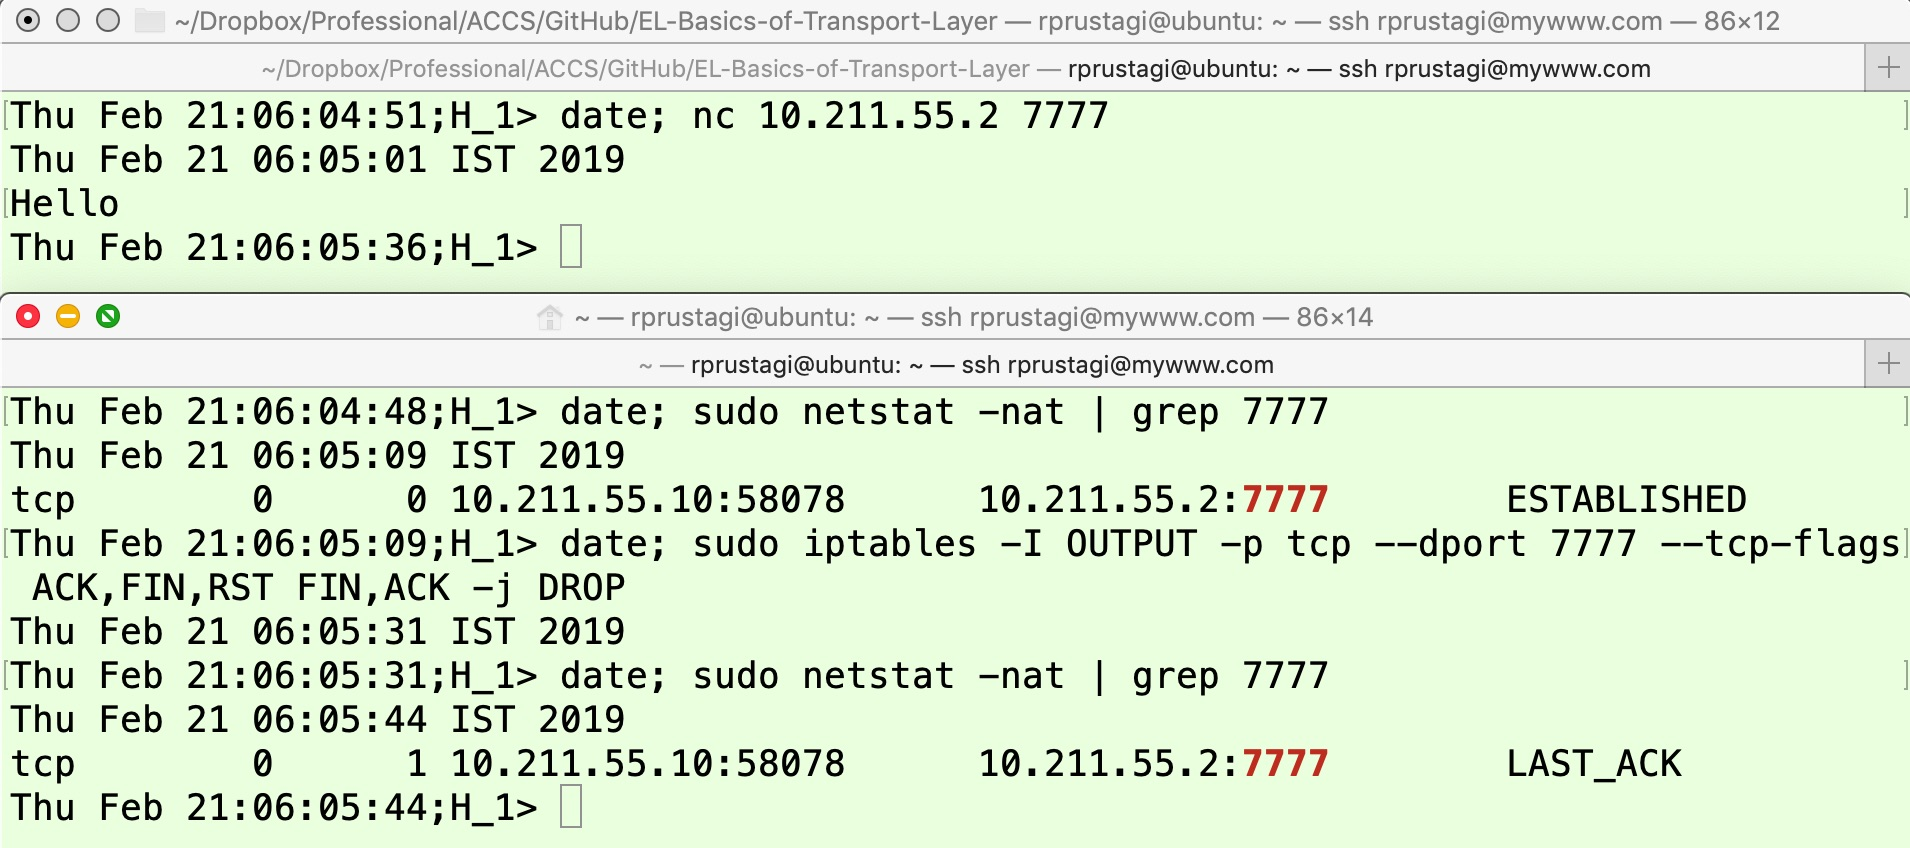
\includegraphics[scale=.22]{src/Figures/chap3/10.jpg}
\caption{Receiving FIN, sending ACK, and FIN-ACK}\label{chap3-fig10}
\end{figure}

\begin{multicols}{2}
\noindent
connection is in CLOSE\_WAIT state has no more data to transmit, the application invokes the \lstinline|close()| call and TCP will send the FIN (3) message and move to the LAST\_ACK state. The originating application that initiated connection close will remain in the FIN\_WAIT2 if the second FIN (3) message is lost, implying network disturbance. Below we describe the experimental exercises to define network conditions depicting the TCP connection states of two communicating applications.

\medskip
\noindent
\textbf{Experiment 5:\\ TCP State FIN\_WAIT2 (\boldmath$H_{2}$) and CLOSE\_WAIT ($H_{1}$)}
\smallskip

We start a netcat server on $H_{2}$. As before, it is necessary to have a client program that continues to send data even after the other side has initiated connection close. Hence, we use the previously described Python client program on $H_{1}$ to establish communication and exchange some data, as shown in the upper panels of Figure \ref{chap3-fig11} and Figure \ref{chap3-fig12}. At this point, the TCP connection is in the ESTABLISHED state as shown by the output of the first command in the lower panel of Figure \ref{chap3-fig12}. The client program \textit{tcp\_client.py} is invoked to send 20 iterations of data transmission (option \textbf{-c}) at an interval of 20 seconds (option \textbf{-d}), and the data transmitted is the current date and time as can been seen in the upper panels of these two figures.

When the \textit{netcat} application is closed on $H_{2}$ at time 11:19:22, it sends a FIN (1) message to $H_{1}$ and moves to the FIN\_WAIT1 state. The application on $H_{1}$ receives this FIN ($1'$) message, responds with ACK (2) and moves to the CLOSE\_WAIT state. Since it has more data to send, it does not send the FIN (3) message and continues to remain in the CLOSE\_WAIT state (as shown by the output of the last command in the lower panel of Figure \ref{chap3-fig12}). However, when $H_{2}$ receives the ACK ($2'$) message, it moves to the FIN\_WAIT2 state as shown in the lower panel of Figure \ref{chap3-fig11} at time 11:19:25.
\end{multicols}

\begin{figure}[!htb]
\centering
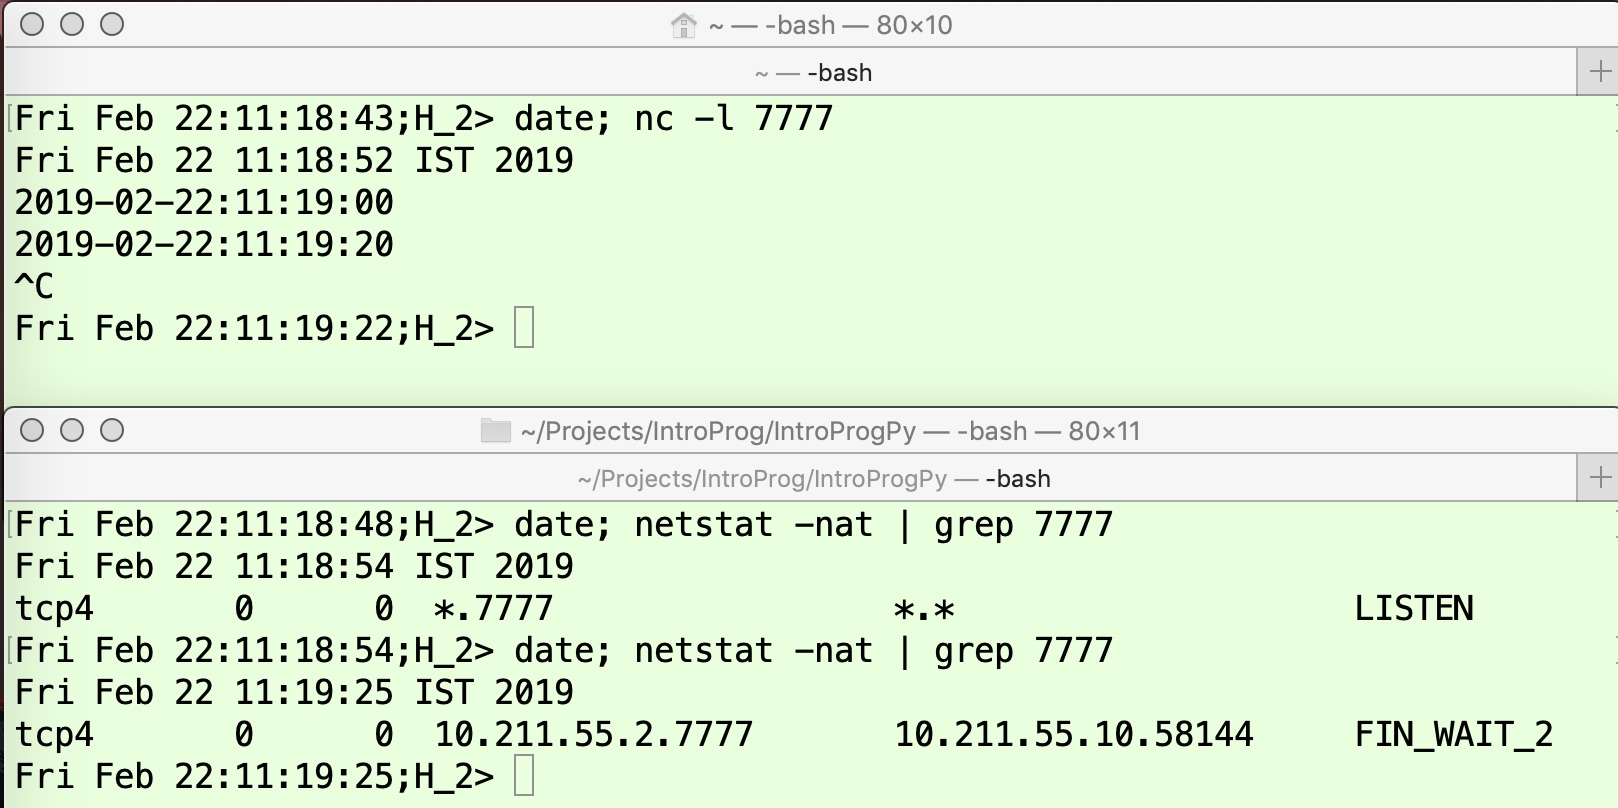
\includegraphics[scale=.23]{src/Figures/chap3/11.jpg}
\caption{FIN\_WAIT2 state while receiving data}\label{chap3-fig11}
\end{figure}

\begin{figure}[!htb]
\centering
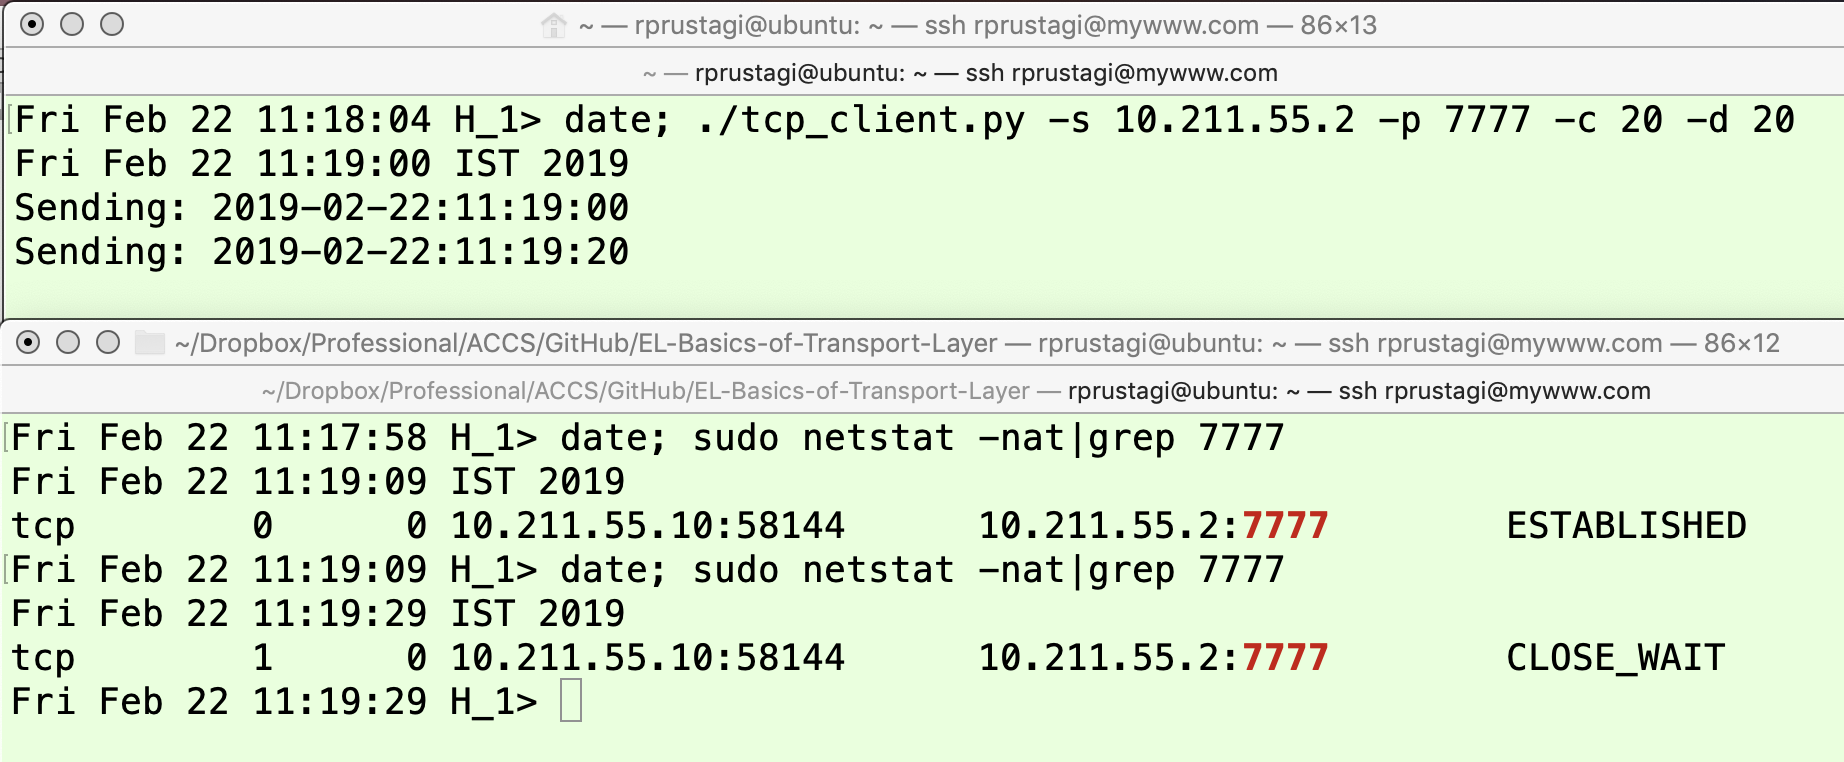
\includegraphics[scale=.45]{src/Figures/chap3/12.jpg}
\caption{CLOSE\_WAIT state while other side initiated close}\label{chap3-fig12}
\end{figure}

\begin{multicols}{2}
\noindent
\textbf{Experiment 6:\\ TCP State FIN\_WAIT2 (\boldmath$H_{2}$) and\hfill\break LAST\_ACK ($H_{1}$)}
\smallskip

In the above experiment, when the FIN (3) message sent by the application on $H_{1}$ does not reach $H_{2}$, then although $H_{1}$ will move the TCP connection state to LAST\_ACK, the state on $H_{2}$ will continue to be FIN\_WAIT2. To realize this situation, one must carefully understand the transitions. When the FIN (1) message sent by $H_{2}$ is received, $H_{1}$ will send the ACK (2) message and move to the CLOSE\_WAIT state. When $H_{2}$ receives this ACK ($2'$) message it will move to the FIN\_WAIT2 state. When $H_{2}$ has finished sending its data, it will send the FIN (3) message that should be lost for the purposes of this experiment. Thus, one must carefully manage the timing of these events as shown in  Figure \ref{chap3-fig13} and Figure \ref{chap3-fig14}.

{\parfillskip=0pt
The TCP application on $H_{1}$ is invoked, which sends 3 data packets starting at time 15:33:35, at an interval of 10 seconds (option \textbf{-d 10}) as shown in the upper panel of Figure \ref{chap3-fig14}. At 15:33:55, the application is aborted on $H_{2}$ (upper panel of Figure \ref{chap3-fig13}), hence the FIN (1) message is sent. Once the ACK (2) message is received, the TCP connection state on $H_{1}$ moves to FIN\_WAIT2, as shown in the lower panel of Figure \ref{chap3-fig13}. The application on $H_{1}$ will wait for 10 more seconds before invoking \lstinline|close()| at 15:34:05. At time 15:34:01, a firewall rule is invoked on $H_{1}$ to drop the FIN\par}
\end{multicols}

\begin{figure}[!htb]
\centering
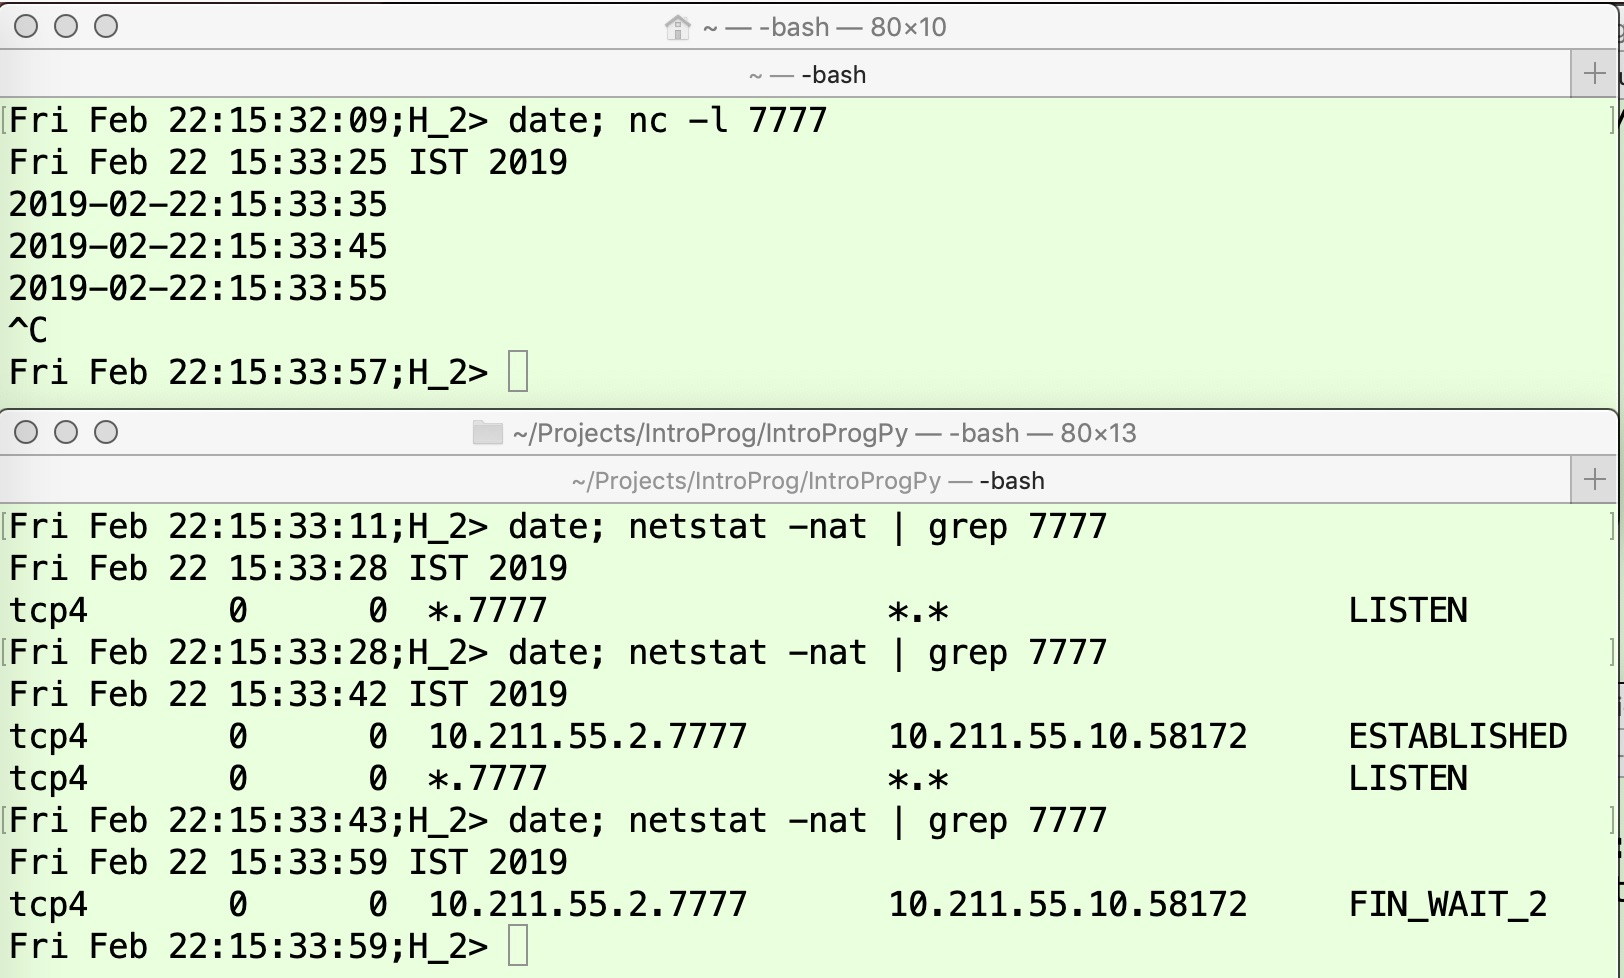
\includegraphics[scale=.22]{src/Figures/chap3/13.jpg}
\caption{FIN\_WAIT2 awaiting FIN from other side}\label{chap3-fig13}
\end{figure}

\begin{figure}[!htb]
\centering
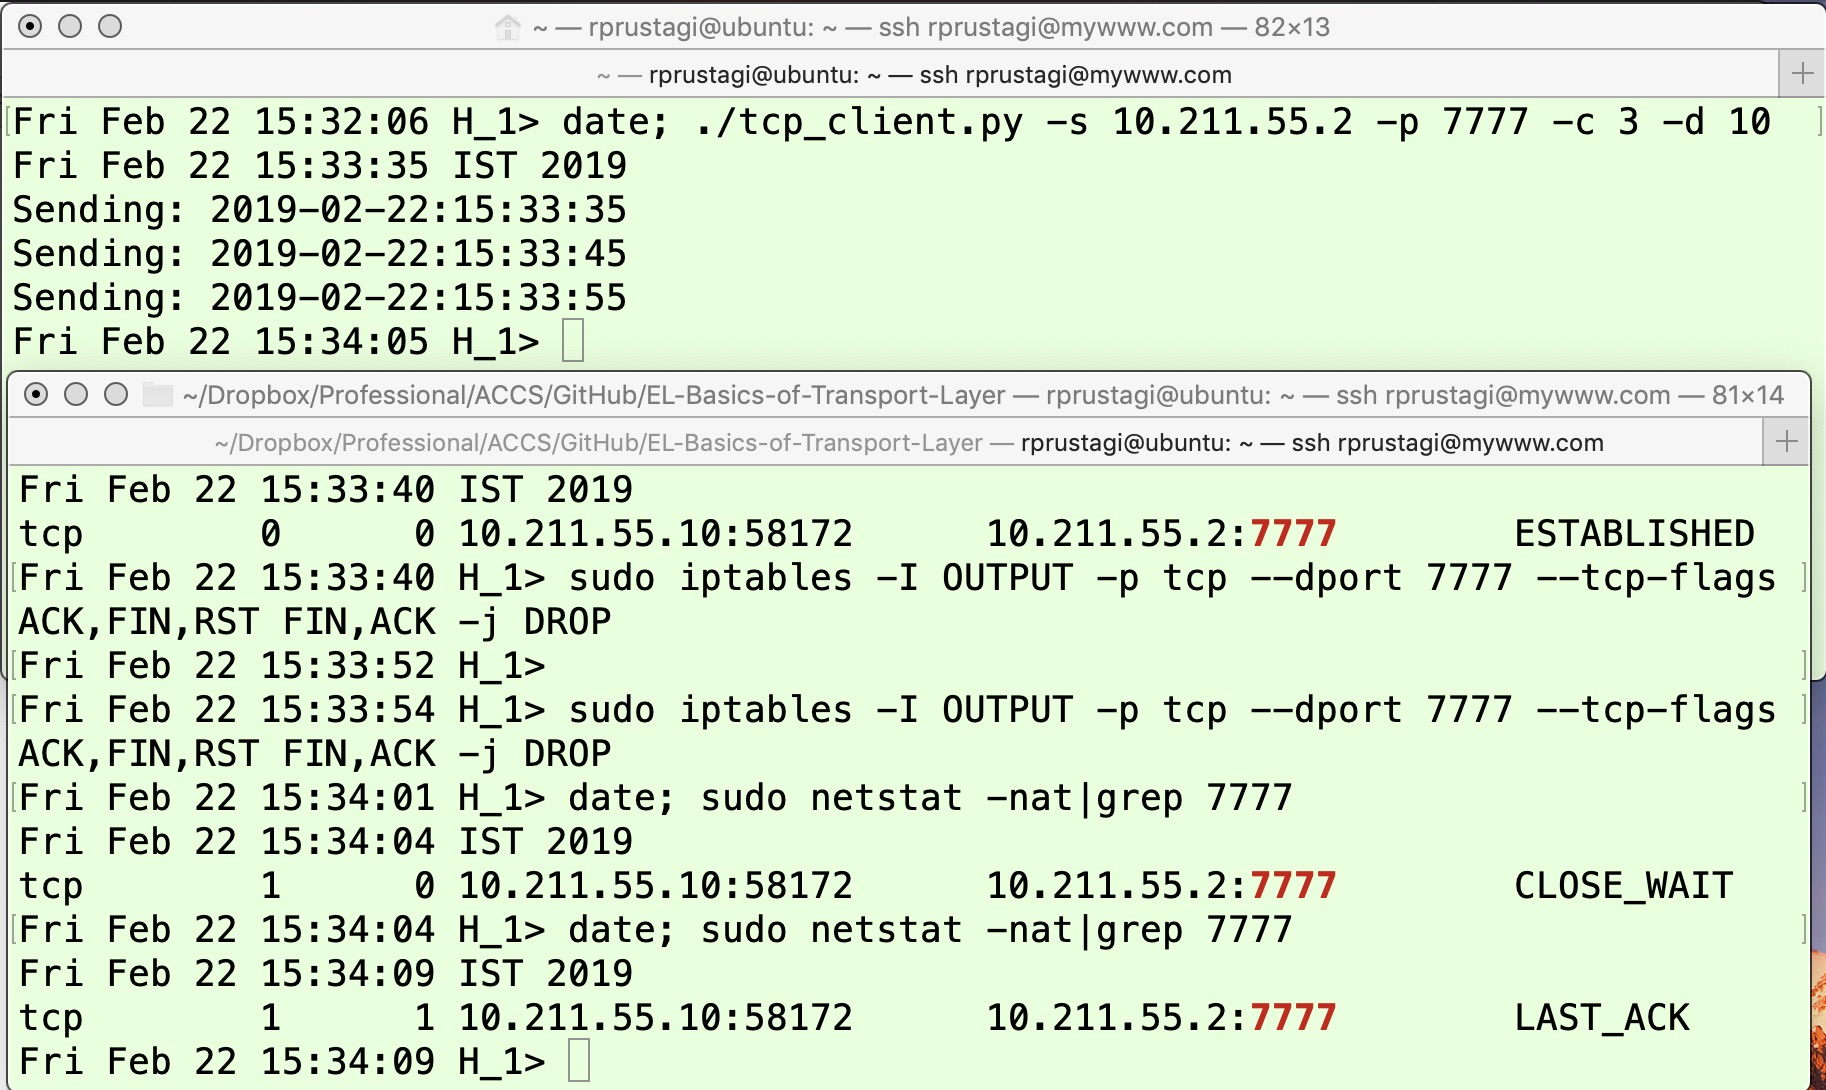
\includegraphics[scale=.21]{src/Figures/chap3/14.jpg}
\caption{Transition from CLOSE\_WAIT to LAST\_ACK}\label{chap3-fig14}
\end{figure}

\begin{multicols}{2}
\noindent
packet, as in the lower panel of Figure \ref{chap3-fig14}. Note that $H_{1}$ has not yet sent the FIN packet -- it is still in the CLOSE\_WAIT state as shown by the output of the fourth command in the lower panel. At time 15:34:05, when the application on $H_{1}$ invokes \lstinline|close()|, it sends the FIN (3) packet and moves to the LAST\_ACK state as shown by the output of the last line in the lower panel of Figure \ref{chap3-fig14}. However, this FIN (3) packet is dropped by the firewall rule, hence it does not reach $H_{2}$. Thus, the state of the TCP connection on $H_{2}$ remains FIN\_WAIT2.

\section{TCP Communication state CLOSING}

You will notice that we have not discussed the CLOSING state. This state is experimentally difficult to observe, because it requires a very high-precision timing of events and is therefore infeasible to create in typical lab scenarios. Thus, we will not define an experimental exercise for this state, but we will describe the general communication scenario that may lead to this state. This state can only be reached when both applications connected by a TCP connection decides to close the connection almost at the same time. Thus, both the applications send the FIN (1) message and move to the FIN\_WAIT1 state awaiting the ACK of its FIN. When in this state, when the first application receives FIN ($1'$) from the second application, it sends the ACK (7) message and moves to the CLOSING state. Similarly, when the second application receives FIN ($1'$) from the first application, it sends the ACK (7) message and moves to the CLOSING state as well. Both applications will receive ACK ($7'$) messages, and they will then move to TIME\_WAIT state.

\section{Summary}

In this paper we have explored the basic workings of the TCP state transition for the teardown phase. We have described these transitions for normal communication and have discussed scenarios that arise when specific network error conditions cause packet-loss during this phase. The timing and nature of packet loss has differing types of impact on the TCP connection state, and states that are normally transient (and difficult to observe) become long-lasting. Network applications that fail to handle such scenarios properly can lead to excessive resource utilization and may suffer from degraded performance. Thus, we hope that the insights into the TCP state transitions provided in this article will be valuable to web developers and devops teams to debug and fix such issues.

The ESTABLISHED state, which corresponds to the data transfer phase of TCP connection, is perhaps the simplest one to understand. In this state, whenever a data packet is received, an acknowledgement is sent back. However, in real life, all performance-related issues for general network communications correspond to this state. Any discussion on TCP communication always entails congestion control and flow control, and both these issues are dealt with in the ESTABLISHED state. These two error-control mechanisms are often (erroneously) perceived to be the same, because the TCP response to both these errors results in same action. In fact, the two error conditions are quite different. Similarly, TCP fairness (the issue of how to allocate bandwidth when a single physical link of limited bandwidth is shared among multiple TCP connections) also corresponds to this state. In our next article, we will discuss the ESTABLISHED state in detail, and aspects of TCP performance or throughput when the network has limited bandwidth or is witnessing packet-loss.

\section{Appendix}

Partial code for TCP client program to demonstrate FIN\_WAIT1, CLOSE\_WAIT and TIME\_WAIT state. The complete program is accessible at \cite{chap3-key10}.
\begin{verbatim}
srvr_addr = (ip_addr, port)
sock = socket.socket(socket.AF_INET, 
                     socket.SOCK_STREAM)
sock.connect(srvr_addr)

for i in range(1,count):
    #msg = chr(64 + i) * buffer + "\n"
    msg = datetime.datetime.now().
	          strftime("%Y-%m-%d:%H:%M:%S")+"\n"
    print "Sending: " + msg,
    sent = sock.send(msg)
    time.sleep(delay
\end{verbatim}

\section{Experiential Exercises}

All the example exercises discussed in this article make use of i) Linux built-in commands related to network utility \textit{nc} for data transfer, ii) \textit{netstat} for monitoring network connection state, and a simple python program (\textit{tcp\_client.py}) to enable timing the packet transmission and respective finer control. If at your Linux installation, the \textit{netstat} utility is not installed, then same can be installed by using the command \lstinline|sudo apt-get install net-tools|. Similarly, the netcat (nc) is available by default on all Linux and Apple Mac machines, and for Windows based systems, there are free open source versions available, which can be downloaded and installed. To develop a lasting understanding, it is suggested that reader should carry out all the experimental exercises. The reader should explore even the different sequencing of steps such as firewall rules, packet loss, etc. to help consolidate the understanding.\raisebox{-.1cm}{
\includegraphics[scale=.9]{src/Figures/circledC.eps}}

\begin{thebibliography}{99}
\bibitem{chap3-key1} RFC 793, ``Transmission Control Protocol'', Information Sciences Institute, USC, CA, Sep 1981, \url{https://tools.ietf.org/html/rfc793}. Last accessed Feb 2019.
\bibitem{chap3-key2} Ram Rustagi, Viraj Kumar, ``Understanding Transport Layer Basics'', ACCS journal of Computing and Communications, Vol 2, Issue 3, Sep 2018. \url{https://acc.digital/experiential-learning-of-networking-technologies-understanding-transport-layer-basics/}, last accessed Feb 2019.
\bibitem{chap3-key3} netstat: man page, \url{http://manpages.ubuntu.com/manpages/bionic/man8/netstat.8.html}, Accessed Feb 2019.
\bibitem{chap3-key4} netstat usage examples: \url{https://www.tecmint.com/20-netstat-commands-for-linux-network-management/}, Accessed Feb 2019.
\bibitem{chap3-key5} Netcat (nc) command utility, \url{http://manpages.ubuntu.com/manpages/xenial/man1/nc.traditional.1.html}, last accessed Feb, 2019.
\bibitem{chap3-key6} nc cheat-sheet, \url{https://www.sans.org/security-resources/sec560/netcat_cheat_sheet_v1.pdf}, last accessed Feb 2019.
\bibitem{chap3-key7} Iptables tutorial. \url{https://www.frozentux.net/iptables-tutorial/iptables-tutorial.html}, last accessed Feb 2019.
\bibitem{chap3-key8} Ram Rustagi, Viraj Kumar, ``Understanding TCP States -- Part I'', ACCS journal of Computing and Communications, Vol 2, Issue 4, Dec 2018; \url{https://acc.digital/experiential-learning-of-networking-technologies-understanding-tcp-states-part-1/}, last accessed Feb 2019.
\bibitem{chap3-key9} Example details for TCP Connection state during connection setup, \url{https://github.com/rprustagi/EL-TCP-States-1.git}. Last accessed Feb 2019.
\bibitem{chap3-key10} Example details for TCP Connection state during tear down phase, \url{https://github.com/rprustagi/EL-TCP-States-2.git}. Last accessed Feb 2019.
\end{thebibliography}
\end{multicols}
